\documentclass{report}
\usepackage[margin=2.5cm]{geometry}
\usepackage{amsmath, amssymb, stmaryrd, latexsym, amsthm, mathtools}
\usepackage{mathpazo, times}
\usepackage{float}
\usepackage{listings}
\usepackage{url}
\usepackage{natbib}
% \usepackage{parskip} % very ugly with lemmas, invariants, etc without intervening text
\usepackage[disable]{todonotes}
\usepackage{slashed}
\usepackage{tikz}
\usetikzlibrary{automata, positioning, arrows}
\tikzset{
    state/.style={
           rectangle,
           rounded corners,
           draw=black, very thick,
           minimum height=2em,
           inner sep=2pt,
           text centered,
           },
}

\usepackage{forest}
\usepackage{IEEEtrantools}
\usepackage{microtype}
\usepackage{graphicx,color}

\usepackage{hyperref}
\hypersetup{
  colorlinks=false,
  linkcolor={blue},
  citecolor={blue},
  urlcolor={blue},
  linkbordercolor={white},
  citebordercolor={white},
  urlbordercolor={white}
}
\usepackage[capitalise,noabbrev,nameinlink]{cleveref}

% https://tex.stackexchange.com/questions/132823/ieeetrantools-clash-with-cleveref
\makeatletter
\let\if@IEEEissubequation\iffalse
\makeatother

\usetikzlibrary{arrows}

\newcommand{\coot}[1]{\textcolor{violet}{\emph{#1}}}
\newcommand{\njd}[1]{\textcolor{purple}{\emph{#1}}}
\newcommand{\avieth}[1]{\textcolor{blue}{\emph{#1}}}
\newcommand{\dcoutts}[1]{\textcolor{orange}{\emph{#1}}}
\addtolength{\marginparwidth}{-0.1\marginparwidth}

\newcommand{\var}[1]{\mathit{#1}}
\newcommand{\type}[1]{\mathsf{#1}}
\newcommand{\powerset}[1]{\mathbb{P}(#1)}
\newcommand{\order}[1]{\mathcal{O}\left(#1\right)}
\newcommand{\restrictdom}{\lhd}
\newcommand{\subtractdom}{\mathbin{\slashed{\restrictdom}}}
\newcommand{\restrictrange}{\rhd}

\newcommand{\hsref}[1]{} % add reference to the relevant Haskell source (as comment)
\newcommand{\wip}[1]{\color{magenta}{#1}\color{black}}
\newcommand{\hide}[1]{}
\newcommand{\trans}[1]{\texttt{#1}}
\newcommand{\state}[1]{\texttt{#1}}
\newcommand{\msg}[1]{\texttt{#1}}
\newcommand{\Idle}{\state{Idle}}
\newcommand{\Busy}{\state{Busy}}
\newcommand{\Done}{\state{Done}}
\newcommand{\MsgDone}{\msg{MsgDone}}

\DeclareMathOperator{\dom}{dom}
\DeclareMathOperator{\range}{range}
\DeclareMathOperator*{\argmin}{arg\,min} % thin space, limits underneath in displays
\DeclareMathOperator*{\minimum}{min}
\DeclareMathOperator*{\maximum}{max}

% Number within sections, and don't have separate counters for separate environments
\theoremstyle{definition}{
  \newtheorem{lemma}{Lemma}[section] % Number within sections
  \newtheorem{definition}[lemma]{Definition}
}
\theoremstyle{theorem}{
  \newtheorem{invariant}[lemma]{Invariant}
  \newtheorem{proofobligation}[lemma]{Proof Obligation}
}

\Crefname{invariant}{Invariant}{Invariants}

\numberwithin{equation}{lemma}

%\floatstyle{boxed}
%\restylefloat{figure}

\lstset{basicstyle=\ttfamily\small}

\raggedbottom

\begin{document}

\title{Data Diffusion and Peer Networking in Shelly\\
       {\small (Version 0.5)} \\
       {\large \sc An IOHK technical report}}
\author{Duncan Coutts \\ {\small \texttt{duncan@well-typed.com}} \\
                         {\small \texttt{duncan.coutts@iohk.io}}
   \and Alex Vieth \\ {\small \texttt{alex@well-typed.com}}
   \and Neil Davies \\ {\small \texttt{neil.davies@pnsol.com}} \\
                       {\small \texttt{neil.davies@iohk.io}}
   \and Marcin Szamotulski \\ {\small \texttt{marcin.szamotulski@iohk.io}}
   \and Karl Knutsson \\ {\small \texttt{karl.knutsson@iohk.io}}
   \and Marc Fontaine \\ {\small \texttt{marc.fontaine@iohk.io}}
   }
%\date{January 25 2019}
\date{\today}

\maketitle

\begin{abstract}
  This document describes .....
\end{abstract}

\tableofcontents

\section*{Version history}

\begin{description}
\item[Version 0.1, Dez 20, 2018  Draft of the table of contents.]
\item[Version 0.2, Jan 08, 2019 Structure and outline.]
\item[Version 0.3, Jan 25, 2019 Start elaborating contents.]
  Description of state machines; Binary representation.
\item[Version 0.4, Jan 28, 2019 Extend state machine description]
\item[Version 0.5, Feb 1, 2019  add PingPong and Block-Fetch protocol]
\end{description}

\chapter{Overview}
\section{Requirements}
\subsection{High level requirements}

These are the high level business requirements for the networking that were
gathered and signed off in late 2017. As such they are expressed in an informal
prose style, and often following a ``user story'' style.

\subsubsection{Network connectivity}

\paragraph{Participate as a user who has delegated}

As a Daedalus home user with my stake delegated to other users I would like to
join the Cardano network so I can participate in the network.
\begin{itemize}
\item The system be designed to provide this user segment with the ability
      to catch up and keep up with the blockchain without having to do any local
      network configuration.
\item The system be designed to provide this user segment with the ability to
      continuously find and maintain a discovery of a sufficient number of
      other network participants that have reasonable connectivity.
\item The system be designed to provide this user segment with the ability to
      find and maintain a minimum of 3 other network participants to maintain
      connectivity with performance that is sufficient to catch up with the
      blockchain.
\item The system design will take into account that this user will probably be
      behind a firewall.
\item Users in the segment can be defined by as having all their stake
      delegated to other network participants.
\end{itemize}


\paragraph{Participate in network as small stakeholder}

As a Deadalus home user operating a core node with a small stake, I would like
to join the Cardano network so I can participate in the network as a core node
that produces blocks i.e. have not delegated to someone else.

\begin{itemize}
\item The system be designed to provide this user segment with the ability to
      receive the transactions that will be incorporated into blocks (although
      sizing the operation of the distributed system to ensure that all such
      participants would be able to receive all transactions is not a bounding
      constraint).
\item The system be designed to provide this user segment with the ability to
      participate in the MPC protocol\footnote{This requirement is now
      redundant because the MPC protocol is specific to Ouroboros Classic.}.
\item The system will be designed to provide this user segment with the ability
      to catch up and keep up with the blockchain without having to do any local
      network configuration (this is a bounding constraint).
\item The user will have sufficient connectivity and performance to receive a
      block within a time slot {\sc and} they have to be able to create and
      broadcast a block within a time slot in which the block is received by
      other core nodes.
\item The system will be designed to maximise the likelihood that 50\% of home
      users operating a core node are compliant with the previous requirement
      at any one time.
\item The system will be designed to provide this user segment with the ability
      to continuously find and maintain a discovery of a sufficient number of
      other network participants that have reasonable connectivity.
\item The system will provide a discovery mechanism that will find and maintain
      a minimum of 3 other network participants to maintain connectivity with
      performance that is sufficient to catch up with the blockchain.
\item The system design will take into account that this user may be behind a
      firewall (i.e being behind a firewall should not preclude a user
      participating in this fashion).
\item The Delegation workstream will provide a UI feature for the user to
      choose to control their own stake.
\item Users in this segment will be defined as {\sc not}
      \begin{itemize}
      \item[a)] being in the top 100 users ranked by stake or
      \item[b)] in a ranked set of users who combined control 80\% of the stake
      \end{itemize}
\item Users in this segment will not be part of the Core Diff, but still
      subject to the normal incentives related to creating blocks.
\end{itemize}


\paragraph{Participate in network as a large stakeholder}

As a user running a core node on a server and with large stake in the network,
I would like to join the Cardano network so I can participate in the network as
a core server node that produces blocks i.e. have not delegated to someone else.

\begin{itemize}
\item A large stakeholder will be defined as
      \begin{itemize}
      \item[a)] being in the top 100 users ranked by stake; or
      \item[b)] in a ranked set of users who combined control 80\% of the stake
      \end{itemize}
\item Assuming that this user has sufficient connectivity and performance, the
      system should ensure that the collective operation of the distributed
      system will ensure that they have a high probability, of receiving a
      block within a time slot such that they have sufficient time to be able
      to create and broadcast a block within a time slot where the block is
      received by other core nodes.
\item It is expected that the previous requirement will be fulfilled to a high
      degree of reliability between nodes in this category -- assuming normal
      network operations

      \begin{tabular}{rl}
      Threshold & $>95\%$ \\
      Target    & $>98\%$ \\
      Stretch   & $>99\%$
      \end{tabular}
\item The system will be designed to provide this user segment with the ability
      to continuously find and maintain a discovery of a sufficient number of
      other network participants that have reasonable connectivity.
\item Discovery will find and maintain a minimum of 10 other network
      participants to maintain connectivity with performance that is sufficient
      to catch up with the blockchain.
\item Ability to receive the transactions that will be incorporated into blocks.
\item Ability to participate in the MPC protocol\footnote{This requirement is
      now redundant because the MPC protocol is specific to Ouroboros Classic.}.
\item The user will catch up and keep up with the blockchain.
\item The server firewall rules will be such that it can communicate with other
      core nodes on the system (and vice versa) -- The system will provide the
      necessary information to update firewall rules if the server is operating
      behind a firewall to ensure the server can communicate with other core
      nodes.
\item The threshold which defines the group of large stakeholders may be
      configurable on the network layer. The configuration may include toggling
      between the rules a) and b) in the previous requirement and the threshold
      numbers within these (this is pending a decision from the Incentives
      workstream.
\item The rules and threshold configuration may need to be a protocol parameter
      that is updated by the update system.
\end{itemize}


\paragraph{Poor network connectivity notification}

As a home user, I want to see a network connection status on Daedalus so that
I know the state of my network connection.
%
\begin{itemize}
\item If the user receives a notification that they are in red or amber mode,
      Daedalus will give the user some helpful information on how to resolve
      common connectivity issues.
\end{itemize}
%
There are three (at least) the following three distinct modes that the network can be operating in:
each one has a red, green, amber status.

%
\begin{center}
\begin{tabular}{ll}
Initial block sync \\
\hline
red   & receiving $<1$ blocks per 10s \\
amber & receiving $<10$ blocks per 10s \\
green & otherwise  \\[1em]

Recovery \\
\hline
red   & receiving $<1$ slot block per 10s \\
amber & otherwise  \\
green & (not applicable) \\[1em]

Block chain following \\
\hline
red   & it has been more that 200s since a slot indication was received. \\
amber & it has been more than 60s since a slot indiction was received. \\
green & otherwise.
\end{tabular}
\end{center}

This assumes that the slot time remains 20 seconds.


\subsubsection{Distributed System Performance}

\paragraph{Transaction Throughput}

The transaction per second of the system as a whole will be:
%
\begin{center}
\begin{tabular}{lr}
Threshold &  8 tps  \\
Target    & 16 tps  \\
Stretch   & 50 tps  \\
\end{tabular}
\end{center}

This assumes that the slot time remains 20 seconds.

\paragraph{Transaction Latency}

As a user I want my transaction to be submitted to the blockchain and received
by the target user within the following time period:
%
\begin{center}
\begin{tabular}{lr}
Threshold & 100 seconds \\
Target    & 60 seconds  \\
Stretch   & 30 seconds  \\
\end{tabular}
\end{center}
%
The above time-frames will be achieved for $>95\%$ of all transactions.

\paragraph{Network Bearer Resource Use -- end user control}

As a user operating on the network as a home user not behind a firewall, I
would like a cap on the total amount of network capacity in terms of short-term
bandwidth that other network users can request from my connection so I am
assured my network resource is not eaten up by the data diffusion function.

\begin{itemize}
\item The cap should be based on a fraction of a typical home internet
      connection -- it can be changed by configuration including ``don't act
      as a super node''.
\item The system will allow users synching with the latest version of the
      blockchain to download blocks from more then one and up to five network
      peers concurrently.
\item A cap on number of incoming subscribers.
\item A cap on number of outbound requests for block syncing from other users.
\item The cap will not be imposed on core nodes running on a server.
\item If these resources are available, a reasonable connection speed should be
      available to users requesting to sync the latest version of the
      blockchain e.g. downloading blocks from 5 peers concurrently to aggregate
      the bandwidth.
\item (nice to have) the actual number and capacity being used is available to
      user.
\end{itemize}

\paragraph{Participant performance measurement}

There may be a requirement for measuring if a large stakeholder is not meeting
their network obligation.

It is accepted that this requirement is a ``nice to have'', and it has not been
established that it is possible, nor has it been incorporated into the
incentives mechanism.

\subsubsection{Distributed System Resilience and Security}

\paragraph{Resilience to abuse}

As a user I should not be able to attack the system using an asymmetric denial
of service attack that will deplete network resources from other users.

\begin{itemize}
\item The system should achieve its connectivity and performance requirements
      even in the presence of a non-trivial proportion of bad actors on the
      network.
\item There is an assumption that there are not a large numbers of bad actors
      in the network.
\item The previous assumption does not follow from the assumptions of Ouroboros
      which states that the users that control 50\% of the stake are
      non-adversarial.
\end{itemize}


\paragraph{DDoS protection}

As a large stakeholder running a core node on a server, I should still be able
to communicate with other user in this segment, even if the system comes under
a DDoS attack.

\begin{itemize}
\item Users in this segment will be able to generate and broadcast blocks to
      each other within the usual timing constraints in this situation.
\end{itemize}

IP addresses will be hidden

\begin{itemize}
\item Encrypted IP addresses will be published by 10 of the other members of
      the group of large stakeholder core nodes.
\end{itemize}

Assumption

\begin{itemize}
\item Core node operators will not publish their IP addresses publicly.
\item Encrypted IP addresses will be published by the 10 of the other members
      of the group of large stakeholder core nodes.
\item If a node operators IP address is compromised the operator will respond
      and change the IP address of their node.
\item The system will allow operators to change the address of their core nodes
      and communicate with that new IP address within a reasonable period of
      time.
\end{itemize}


\subsubsection{Network decentralization}

\paragraph{No hegemony}

As a user I want to be assured that IOHK and its business partners are not in
an especially privileged position in terms of trust, responsibility and
necessity to the network so that network hegemony is avoided.

\begin{itemize}
\item IOHK should be in the same position on the network as any other
      stakeholder with an equivalent amount of stake.
\item There is more general requirement that no other actor could do this
      either.
\end{itemize}

\section{Context and Introduction}

How this work relates (in general terms) to the rest of the Shelly
development and the Ourbouros papers.

\subsection{Data Diffusion assumptions in Ourbouros}
\begin{quote}
  This is the ``telling them what you are going to tell them'' part -
  outline of the data diffusion and overlay network bringing out the
  key functional and non-functional relationships - aim to serve as a
  general executive overview as well as a framing of PoS issues.
\end{quote}
\begin{itemize}
  \item Assumptions of the mathematical model(s)
  \item Goal of the data diffusion functionality
  \item Strong requirement on collective performance
  \begin{itemize}
    \item Chain growth quality
    \item Adverserial actor assumption
  \end{itemize}
\end{itemize}
\subsection{Functional Layering}
pictures as to how the various functional layers relate; How the Data
diffustion layer relates to Ledger etc; How data diffusion relates to
point-to-point overlay network.

\subsubsection{Non-function aspects}
Performance; trustworthiness; Forwarding as an expression of confirmed
``trust'' (and corollary - forwarding of \emph{clearly} incorrect information
seen as prima-facia evidence of adversarial action.
\subsection{Protocol Roles}
Peer relationship between various nodes; Limited trust and
verification; (Brief) description of the expectations and assumptions across
the functionality boundaries; 

\subsubsection{Mini Protocols}
\begin{description}
\item[Chain Tip Following] (or whatever the agreed name is)
\item[Bulk Chain Download] ....
\item[Transaction Difussion] ....
\item[$\Delta Q$ Measurement] (not really an mini protocol, in that it
  is point to point and not part of the diffusion process itself,
  placed here because it ``sits'' on top of the overlay network. Role
  to generate active endpoint performance data to help optimise
  time-to-diffuse critical information exchanges (e.g. newly minted
  block diffusion)
\end{description}  
\subsubsection{Point to point Overlay Network}
need picture; note that long term eclipse attacks are not an issue
here (cover why a bit later); tie in chain growth requirements with
need for ``better'' communications performance between (major)
stakepools (notion of Core DIF); association explain need for
\begin{itemize}
\item fixed configuration (with/without others from this list)
\item Core DIF
\item Distributed endpoint discovery (subset of notion of peer in
  other approaches)
\end{itemize}

  
\section{Layout of the Document}

\begin{itemize}
  \item What goes in which section ?
  \item In which order to read ?
  \item Which sections can be skipped ?
\end{itemize}

\section{Notation}

\chapter{Requirements}

\section{Performance Requirements and User Stories}
\subsection{Classes of Participants}
\wip{todo: make a nice table}

\subsubsection{Stake pool} % lookup what this is called in the protocols.tex
\subsubsection{Small stakeholder}
\subsubsection{User who has delegated}
\subsubsection{Requirements for Participants}
\subsubsection{Requirements for Stake Pools}
\subsubsection{Services that the System should provide}

There are two kinds of Requirements:

\begin{enumerate}
\item System capabilities for a node to take a blockchain slot creation role in the protocol.
\item What services that the system provides to the user.
\end{enumerate}



\section{Protocol Updates on the Blockchain}
\begin{itemize}
\item Hybrid phase of federation and decentralization
\item Gradually transition between protocol variants on a life blockchain.
\item Several protocol variant active in parallel.
\item Communication between Shelley Nodes and existing core nodes.
\end{itemize}

\section{Node to Node and Node to Consumer IPC}
There are two basic variants of inter-process-communication in the network:
\begin{itemize}
\item IPC between Cardano nodes that are engaged in the high level Ouroboros
      blockchain consensus protocol.
\item IPC between a Cardano node and a `chain consumer' component such as a
      wallet, explorer or other custom application.
\end{itemize}
Both variants of IPC in the network follow distinct requirements and constraints, and
,while the first version of Cardano used a single protocol, the new version will
use different sets of protocols for both uses cases.
(See Section~\ref{why_distinguish_protocols} for the motivation for this design decision.)
Throughout the document it will be clear which variant of we are referring to.

\section{Threat Model}
\wip{
  WIP discussion of the threat model
\subsection{Resource Consumption Attacks}
}

\section{Ouroboros}
\wip{
How PoS is different from PoW in its network requirements:
}

\begin{itemize}
  \item No capability to sustain an undetected Eclipse attack
  \item Sustained liveness requirement
\end{itemize}

\section{Delegation}


\chapter{Infrastructure}
\label{infrastructure}
\wip{
  WIP: Specific assumptions about the infrastructure that are relevant for the discussion.
}

\section{Internet}
\section{Network Topology}
\section{Topographical distribution of block creating nodes}
\section{TCP}
\section{Operating Systems}
\section{Firewall}
\section{Nodes and Hosting}


\chapter{System Architecture}
\section{Overview}

Traditionally network protocols are presented as a stack of layers where
upper layers build on services provided by lower layers and lower layers
are agnostic of the implementation of the upper layers.
This concept of layers is misleading when discussing Shelly.
It is {\em not} the case that the consensus (layer) is build on top of the network (layer).
It is more appropriate to talk about a network component than a network layer.
The network component provides services to the consensus component and vice versa.
The network component uses the consensus component to carefully validate every piece of
information that it distributes to other nodes.
This is essential to guard against certain kinds of DoS attacks.
This is also the reason why the network component in Shelly cannot be replaced
with an of-the-shelf peer-to-peer protocol.

\section{Design Choices}
\wip{
\begin{itemize}
\item Only the design choices that have been taken.
\item In this section only the big design choices.
\item Design discussions and details in the discussions section.
\end{itemize}
}

\section{Nodes}
\subsection{Node Components}

\begin{figure}[h]
  \pgfdeclareimage[height=10cm]{node-diagram-chains-state}{node-diagram-concurency.pdf}
  \begin{center}
    \pgfuseimage{node-diagram-chains-state}
  \end{center}
  \caption{Data flow inside a Node}
  \label{node-diagram-concurency}
\end{figure}

\chapter{Protocols}
\section{Protocols as State-machines}
The reference implementation of several sub-protocols uses a generic framework
for state-machines.

A Haskell implementation of the state machine framework is described in
Section~\ref{Haskell-state-machine}. It uses correct by construction
techniques to guarantee
several properties of the protocol and the implementation.
In particular it guarantees that there are no deadlocks. At any time, one side has agency
(is expected to transmit the next message) and the other side is waiting for the message,
or both sides agree the protocol has terminated.
The transmission of a message that is not expected by the protocol aborts the execution
of the protocol.

For each sub-protocol that is based on this underlying framework, the description provides the
following pieces of information:

\begin{itemize}
\item An informal description of the protocol.
\item States of the state-machine
\item The messages that are exchanged
\item A transition graph of the global view of the state machine.
\item The client implementation of the protocol.
\item The server implementation of the protocol.
\end{itemize}

\begin{description}
\item[State Machine]
  The Protocols are described as a state machine.
  The specification uses different representations of the state machine,
  for example transition tables or diagrams, that all describe the same protocol.

\item[States]
  We need to distinguish between the global state of a system,
  which includes the values of all local variable stored on the nodes,
  and the abstract states of the state machines.
  The abstract states are equivalent classes of the global state.
  Every global state belongs to exactly one abstract state.
  This specification describes the state machine in terms of the abstract states.
  By definition, client and server are always in identical states
  which also means that client and server simultaneously transit to new states.
  The concrete implementation needs to relax the definition of the abstract state.
  In the concrete implementation the abstract view of state is replaced with
  client state and server state and transitions on either side happens independently
  when a message is either send or received.
  While a message is in-flight the state of the receiver is undefined.
  The state determines which side is active the client or the server.
  
\item[Messages/Events]
  Messages are elements from the set
  $\{(lable, data) \mid lable \in Labels, data \in Data\}$.
  Protocols use a small set of $Lables$ typically $|Labels| \leq 10$.
  State-machine frame work requires that messages can be serialized,
  transferred over the network and de-serialized by the receiver.
  The binary format for messages is described in Section~\ref{CBOR-section}.

\item[Transitions]
  This part of the document describes the transitions of the abstract state of the protocol
  as the result of messages passed between client and the server.
  In sync with abstract state the client and the server update the local data
  to compute the actual "outcome" of a protocol-run, for example "update the
  blockchain".
  \wip{WIP: there are also hard contraints on the transitions, e.g. transaction is valid,etc}

\item[Agency]
  A node has agency if it is expected to send the next message.
  In every state (except the \Done state) either the client or server has agency
  In \Done state the protocol has terminated and neigther side is expected to send any more messages.

\item [State machine transition diagram]
      In state machine diagrams states are drawn as circles.
      States with agency at the client are drawn in green, states with agency at the server in blue and
      the \Done-state in black.
      By construction the system is always in exactly one state,
      i.e. the client is always in the same state as the server,
      regardless of which color the state is drawn in.
      It is also important to understand, that the arrows in the state transition diagram denote
      state transitions and not the direction of the message that is being transmitted.
      This may be confusing because the arrows are labeled with the messages and
      many arrows go from a green state to a blue state or vice versa.

      \wip{TODO: find a latex style to mark tricky sections that must be read carefully.}

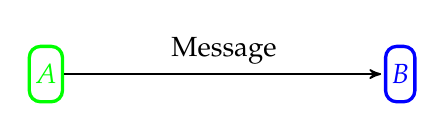
\begin{tikzpicture}[->,>=stealth',shorten >=1pt,auto,node distance=4.5cm, semithick]
  \tikzstyle{every state}=[fill=red,draw=none,text=white]
  \node[state, green]              (A)      {$A$};
  \node[state, blue ,right of=A]   (B)      {$B$};
  \draw (A)            edge[above]          node{Message}   (B);
\end{tikzpicture}

      $A$ is green, i.e in state $A$ the client has agency.
      Therefore the client sends a message to the server and
      both client and server transition to state $B$.
      As $B$ is blue the agency also changes from client so server.

\begin{tikzpicture}[->,>=stealth',shorten >=1pt,auto,node distance=4.5cm, semithick]
  \tikzstyle{every state}=[fill=red,draw=none,text=white]
  \node[state, blue]               (C)      {$C$};
  \node[state, blue ,right of=A]   (D)      {$D$};
  \draw (A)            edge[above]               node{Message}   (B);
\end{tikzpicture}

      $C$ is blue, i.e in state $C$ the server has agency.
      Therefore the server sends a message to the client and
      both client and server transition to state $D$.
      As $D$ is also blue the agency remains at the server.
      The arrows, in the diagrams above,
      cannot be interpreted as a message being send from $A$ to $B$ or from $C$ to $D$.

\item[Client and server implementation]
  The state machine describes which messages are send and received and in which order.
  This is the external view of the protocol that every compatible implementation MUST follow.
  In addition to the external view of the protocol, this part of the specification also describes
  how the client and server actually process the transmitted messages,
  i.e., how the client and server update their internal state upon the transmission of messages.

  This part gives a high level mathematical description, that is useful for understanding the design
  of the protocol itself,
  but does not restrict a concrete implementation of the protocol to specific data structures
  or implementation techniques.
  \wip{
    Operational semantic/ inference rule -style formalism? <- not good,
    but there are even more side-effects !
    there are many mini protocols running in parallell and many layers of abstraction
    imperative update-style !
  }
\end{description}

\section{Ping-Pong Protocol}
\label{ping-pong-protocol}
\hsref{typed-transitions/src/Protocol/PingPong/Type.hs}
\newcommand{\Ping}{\msg{Ping}}
\newcommand{\Pong}{\msg{Pong}}

\subsection{Description}
A client can use the Ping-Pong protocol to check that the server is responsive.
The Ping-Pong protocol is very simple, because the messages do not carry any data and
because the Ping-Pong client and the Ping-Pong server to not access the internal state of the node.
The Ping-Ping protocol uses the same framework for state-machines as the other protocols,
but because the protocol is so simple, the description of the protocol is also very simple and slightly
different that the descriptions of the other protocols.

\subsection{State Machine}

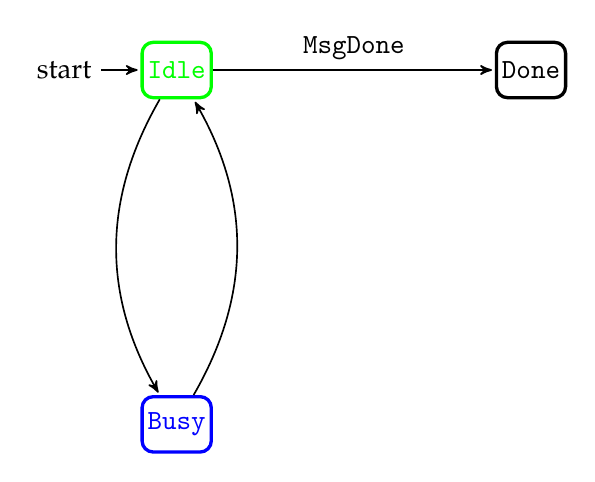
\begin{tikzpicture}[->,>=stealth',shorten >=1pt,auto,node distance=4.5cm, semithick]
  \tikzstyle{every state}=[fill=red,draw=none,text=white]
  \node[state, green, initial]                            (Idle)      {\Idle};
  \node[state, right of=Idle]                             (Done)      {\Done};
  \node[state, blue, below of=Idle]                       (Busy)      {\Busy};

  \draw (Idle)         edge[above]               node{\MsgDone}                  (Done);
  \draw (Idle)         edge[left, bend right]    node{\Ping}                     (Busy);
  \draw (Busy)         edge[right, bend right]    node{\Pong}                     (Idle);
\end{tikzpicture}

Agency:

\begin{figure}[H]
\begin{tabular}{|l|l|} \hline
  Client has Agency & \Idle \\  \hline
  Server has Agency & \Busy \\  \hline
\end{tabular}
\end{figure}

The protocol uses the following messages.
The messages of the Ping-Pong protocol do not carry any data.
\wip{Todo: there is no CBOR codec for the Ping-Pong protocol messages in the sources only a String codec.}
\begin{description}
\item [\Ping]
      The client sends a Ping request to the server.
\item [\Pong]
      The server replies to a Ping with a Pong.
\item [\MsgDone]
      Terminate the protocol.
\end{description}

Transition table:

\begin{tabular}{|l|l|l|}
  \hline
  \multicolumn{3}{|c|}{Transitions} \\ \hline
  from state   & message/event      & to state    \\ \hline\hline
  \Idle        & \Ping              & \Busy   \\ \hline
  \Busy        & \Pong              & \Idle   \\ \hline
  \Idle        & \MsgDone           & \Done       \\ \hline
\end{tabular}

\section{Single Phase Chain Synchronization Protocol}
\label{chain-sync-protocol}
\hsref{ouroboros-network/src/Ouroboros/Network/Protocol/ChainSync/Type.hs}
\newcommand{\CanAwait}{\state{CanAwait}}
\newcommand{\MustReply}{\state{MustReply}}
\newcommand{\Intersect}{\state{Intersect}}
\newcommand{\RequestNext}{\msg{RequestNext}}
\newcommand{\AwaitReply}{\msg{AwaitReply}}
\newcommand{\RollForward}{\msg{RollForward}}
\newcommand{\RollBackward}{\msg{RollBackward}}
\newcommand{\FindIntersect}{\msg{FindIntersect}}
\newcommand{\IntersectImproved}{\msg{IntersectImproved}}
\newcommand{\IntersectUnchanged}{\msg{IntersectUnchanged}}

\subsection{Description}
The chain synchronization protocol is used by the blockchain consumer
to replicate the producer's blockchain locally. As it is polymorphic in blocks,
it supports a family of Ouroboros protocols.
The chain synchronization protocol is used by clients which synchronize just headers (node-to-node),
and also clients which synchronize actual the blockchain (e.g., node-to-wallet).
(See Figure~\ref{node-diagram-concurency}.)

\hide{
\begin{description}
\item[Who is communicating]
  A node communicates with several upstream and downstream nodes.
  The node runs independent agents for every other node
  it communicates with, whether it acts as an upstream or a downstream peer.
\end{description}
}

\subsection{State Machine}

\subsubsection{Sate Machine Diagram}

Agency:

\begin{figure}[H]
\begin{tabular}{|l|l|} \hline
  Client has Agency & \Idle \\  \hline
  Server has Agency & \CanAwait, \MustReply, \Intersect \\ \hline
\end{tabular}
\end{figure}

\begin{tikzpicture}[->,>=stealth',shorten >=1pt,auto,node distance=4.5cm, semithick]
  \tikzstyle{every state}=[fill=red,draw=none,text=white]
  \node[state, green, initial]                            (Idle)      {\Idle};
  \node[state, right of=Idle]                             (Done)      {\Done};
  \node[state, blue, below left of=Idle]                  (CanAwait)  {\CanAwait};
  \node[state, blue, right of=CanAwait]                   (MustReply) {\MustReply};
  \node[state, blue, above of=Idle]                       (Intersect) {\Intersect};

  \draw (Idle)         edge[left, bend right]      node{\RequestNext}           (CanAwait);
  \draw (CanAwait)     edge[above, bend right]     node{\AwaitReply}            (MustReply);
  \draw (CanAwait)     edge[above,bend right=45]     node{\RollForward}           (Idle);
  \draw (MustReply)    edge[right,bend right=45]     node{\RollForward}           (Idle);
  \draw (CanAwait)     edge[above,bend right=80]     node{\RollBackward}          (Idle);
  \draw (MustReply)    edge[right,bend right=80]     node{\RollBackward}          (Idle);
  \draw (Idle)         edge[right, bend right]    node{\FindIntersect}         (Intersect);
  \draw (Intersect)    edge[above, bend right=45]    node[below = 4mm]{\IntersectImproved}     (Idle);
  \draw (Intersect)    edge[above, bend right=80]    node[above = 4mm]{\IntersectUnchanged}    (Idle);
  \draw (Idle)         edge[above]                node{\MsgDone}                  (Done);

\end{tikzpicture}

The protocol uses the following messages:
\begin{description}
\item [\RequestNext]
      Request the next update from the producer.
      The response can be a roll forward, a roll back or wait.
\item [\AwaitReply]
      Acknowledge the request but require the consumer to wait for the next update.
      This means that the consumer is synced with the producer, and
      the producer is waiting for its own chain state to change.
\item [\RollForward~{\boldmath $(header,point)$}]
      Tell the consumer to extend their chain with the given $header$.
      The message also tells the consumer about the $head$ point of the producer.
\item [\RollBackward~{\boldmath $(point_{old},point_{head})$}]
      Tell the consumer to roll back to a given $point_{old}$ on their chain.
      The message also tells the consumer about the new head $point_{head}$ of the producer.
\item [\FindIntersect~{\boldmath $\langle point \rangle $}]
      Ask the producer to try to find an improved intersection point between
      the consumer and producer's chains.
      The consumer sends a sequence {\boldmath $\langle point \rangle $}
      and it is up to the producer
      to find the first intersection point on its chain and send it back to the consumer.
\item [\IntersectImproved~{\boldmath $(point_{intersect},point_{head})$}]
      The reply to the consumer about an intersection found, but {\bf only} if this
      is an improvement over previously established intersection point.
      The consumer can decide weather to send more points.
      The message also tells the consumer about the head point of the producer.
\item [\IntersectUnchanged~{\boldmath $(point_{head})$}]
      The reply to the consumer that no intersection was found: none of the
      points the consumer supplied are on the producer chain.
      The message also tells the consumer about the head point of the producer.
\item [\MsgDone]
      Terminate the protocol.
\end{description}

Transition table:

\begin{tabular}{|l|l|l|l|}
  \hline
  \multicolumn{4}{|c|}{Transitions} \\ \hline
  from state   & message/event      & parameter              & to state    \\ \hline\hline
  \Idle        & \RequestNext        &                        & \CanAwait   \\ \hline
  \Idle        & \FindIntersect      & $points$               & \Intersect  \\ \hline
  \Idle        & \MsgDone            &                        & \Done       \\ \hline
  \CanAwait    & \AwaitReply         &                        & \MustReply  \\ \hline
  \CanAwait    & \RollForward        & $header$,$point$       & \Idle       \\ \hline
  \CanAwait    & \RollBackward       & $header$,$point$       & \Idle       \\ \hline
  \MustReply   & \RollForward        & $header$,$point$       & \Idle       \\ \hline
  \MustReply   & \RollBackward       & $point$,$point$        & \Idle       \\ \hline
  \Intersect   & \IntersectImproved  & $point_1$,$point_2$    & \Idle       \\ \hline
  \Intersect   & \IntersectUnchanged & $point$                & \Idle       \\ \hline

\end{tabular}

\subsection{Client Implementation}

\subsection{Server Implementation}
\wip{TODO: the part in protocol.tex that explains Figure~\ref{chain-diagram-read-pointers}.}
\begin{figure}[h]
\pgfdeclareimage[height=6cm]{chain-diagram-read-pointers}{chain-diagram-read-pointers.pdf}
\begin{center}
\pgfuseimage{chain-diagram-read-pointers}
\end{center}
\caption{Representation of a producer's chain, including `read pointers' for two example consumers.}
\label{chain-diagram-read-pointers}
\end{figure}

\section{Block Fetching}
\label{block-fetching-protocol}
\hsref{ouroboros-network/ouroboros-network/src/Ouroboros/Network/Protocol/BlockFetch2/Type.hs}
\hsref{branch coot/block-fetch-v2}
\subsection{Description}
\renewcommand{\Idle}{\state{Idle}}
\renewcommand{\Busy}{\state{Busy}}
\newcommand{\Streaming}{\state{Streaming}}
\renewcommand{\Done}{\state{Done}}
\newcommand{\RequestRange}{\state{RequestRange}}
\newcommand{\StartBatch}{\state{StartBatch}}
\newcommand{\NoBlocks}{\state{NoBlocks}}
\newcommand{\Block}{\state{Block}}
\newcommand{\BatchDone}{\state{BatchDone}}
\newcommand{\ClientDone}{\state{ClientDone}}

The block fetching mechanism enables a node to download a range of blocks.

\begin{description}
\item[Purpose of the protocol]

\end{description}

\begin{description}
\item [\RequestRange~{\boldmath $range$}]
  The client requests a {\boldmath $range$} of blocks from the server.
\item [\NoBlocks]
  The server tells the client that it does not have blocks.
\item [\StartBatch]
  The server starts block streaming.
\item [\Block~{\boldmath $body$}]
  Stream a single block.
\item [\BatchDone]
  The server ends block streaming.
\item [ClientDone]
  The client terminates the protocol.
\end{description}

\subsection{State machine}

\begin{tikzpicture}[->,>=stealth',shorten >=1pt,auto,node distance=4.5cm, semithick]
  \tikzstyle{every state}=[fill=red,draw=none,text=white]
  \node[state, green, initial]                            (Idle)      {\Idle};
  \node[state, right of=Idle]                             (Done)      {\Done};
  \node[state, blue, below left of=Idle]                  (Busy)      {\Busy};
  \node[state, blue, right of=CanAwait]                   (Streaming) {\Streaming};

  \draw (Idle)         edge[above]                node{\ClientDone}                  (Done);
  \draw (Idle)         edge[left,bend right]      node{\RequestRange}                (Busy);
  \draw (Busy)         edge[above,bend right]     node{\NoBlocks}                    (Idle);
  \draw (Busy)         edge[above]                node{\StartBatch}                  (Streaming);
  \draw (Streaming)    edge[loop right]           node{\Block}                       (Streaming);
  \draw (Streaming)    edge[right]                node{\BatchDone}                   (Idle);
\end{tikzpicture}

Agency:

\begin{tabular}{|l|l|} \hline
  Client has Agency & \Idle            \\  \hline
  Server has Agency & \Busy, \Streaming \\ \hline
\end{tabular}

Transition table:

\begin{tabular}{|l|l|l|l|}
  \hline
  \multicolumn{4}{|c|}{Transitions} \\ \hline
  from state   & message/event       & parameter              & to state    \\ \hline\hline
  \Idle        & \ClientDone         &                        & \Done       \\ \hline
  \Idle        & \RequestRange       & $range$                & \Busy       \\ \hline
  \Busy        & \NoBlocks           &                        & \Idle       \\ \hline
  \Busy        & \StartBatch         &                        & \Streaming  \\ \hline
  \Streaming   & \Block              & $body$                 & \Streaming  \\ \hline
  \Streaming   & \BatchDone          &                        & \Idle       \\ \hline
\end{tabular}

\wip{Todo implement: CBOR codec for block fetch}

\section{Request Response Protocol}
\label{request-response-protocol}
\subsection{Description}
The request response protocol is polymorphic in the request and response data that is been transmitted.
This means there different possibe applications of this protocol and the
application of the protocol determins the type of the requests and responses.

\begin{description}
\item[Purpose of the protocol]
  Nodes use the request response protocol to forward transactions that have been
  submitted to the network.
\end{description}

\subsection{State machine}
\hsref{ouroboros-network/src/Ouroboros/Network/Protocol/ReqResp/Type.hs}
\begin{figure}[H]
\begin{tabular}{|l|l|}
  \hline
  \multicolumn{2}{|c|}{States} \\ \hline
  Name  & Agency \\ \hline \hline
  Idle       & client \\ \hline
  Busy   & server \\ \hline
  Done       &        \\ \hline
  \hline
\end{tabular}
\end{figure}

\begin{figure}[H]
\begin{tabular}{|l|l|l|l|}
  \hline
  \multicolumn{4}{|c|}{Transitions} \\ \hline
  message/event      & parameter              & from        & to       \\ \hline\hline
  Request            & $request$              & Idle        & Busy      \\ \hline
  AwaitReply         & $response$             & Busy        & Done \\ \hline
\end{tabular}
\end{figure}

\begin{figure}[H]
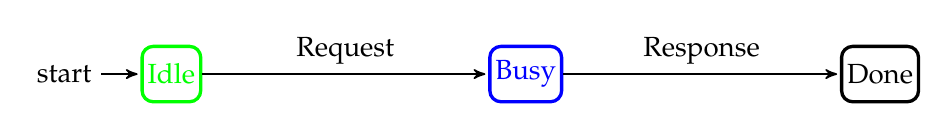
\begin{tikzpicture}[->,>=stealth',shorten >=1pt,auto,node distance=4.5cm, semithick]
  \tikzstyle{every state}=[fill=red,draw=none,text=white]
  \node[state, green, initial]                                   (Idle)      {Idle};
  \node[state, blue, right of=Idle]                              (Busy)      {Busy};
  \node[state, right of=Busy]                                    (Done)      {Done};

  \draw (Idle)         edge[]      node{Request}           (Busy);
  \draw (Busy)         edge[]      node{Response}          (Done);

\end{tikzpicture}
\end{figure}

\section{DeltaQ Mini Protocol}
\wip{
  WIP : Explain DeltaQ measurement backpressure and how we deal with slow connection.
  also See Section \ref{deltaq-discussion}.
The DeltaQ mini protocol does not transmit is own messages.
Instead it relies on the time stamps that the mutiplexing layer (Section~\ref{multiplexing}) adds
to the messages of other mini protocols.
}

\section{Running many Instances of a Mini Protocol in parallel}
\wip{WIP Pipelining}

\section{Multiplexing multiple Mini Protocols over one Channel}
\label{multiplexing}
The multiplexing protocol is used to run several mini protocols in parallel over a single
channel.
The implementation of the mini protocol performs the following tasks:
\begin{itemize}
\item
  It queues outgoing messages from the mini protocols.
\item
  It selects a message for transmission, wraps the message in a multiplexing frame
  and transmits forwards the frame.
\item
  It receives frames from the channel unpacks the frames and dispatches
  the messages to the mini protocols
\item
  It collects the DeltaQ measurements for the DeltaQ Mini Protocol.
\item
  It initializes and terminates channels.
\item
  When a mini protocol detects that the peer violates the protocol, it takes appropriate action,
  i.e. shutdown or abort the channel.
\end{itemize}

\subsection{Multiplexing Frames}
The multiplexing frame adds two 32-bit words to the payload.

\begingroup
\setlength{\tabcolsep}{3pt}
\begin{tabular}{|c|c|c|c|c|c|c|c|c|c|c|c|c|c|c|c|c|c|c|c|c|c|c|c|c|c|c|c|c|c|c|c|}
  \hline
  0&1&2&3&4&5&6&7&8&9&0&1&2&3&4&5&6&7&8&9&0&1&2&3&4&5&6&7&8&9&0&1 \\ \hline
  \multicolumn{32}{|c|}{transmission time} \\ \hline
  \multicolumn{1}{|c|}{M}
  &\multicolumn{15}{|c|}{mini protocol ID}
  &\multicolumn{16}{|c|}{length} \\ \hline
  \multicolumn{32}{|c|}{} \\
  \multicolumn{32}{|c|}{payload} \\
  \multicolumn{32}{|c|}{} \\ \hline
\end{tabular}
\endgroup

\chapter{Peer Discovery and Peer Selection}
\wip{
  Peer discovery and peer selection are relatively independent for the core components of a node.
  In a first iteration, it may be enough to specify what data is going from
  the peer selection algorithm to
  the core components and what data is going from the core components to the peer selection.
  Also peer discovery and peer selection are relatively independent from each other.
  }

\chapter{Haskell}
While the network protocol itself can be implemented in many programming languages,
it has been developed in parallel with a Haskell reference implementation.
In addition to the language agnostic protocol description in the other parts of this document,
this section discusses key aspects of the Haskell implementation.
This section is most useful for people who work with the Haskell reference implementation and
may give some extra insights for anybody who is interested in implementing the
network component.
For understanding the protocol, it is save to skip this section.
\begin{figure}
\pgfdeclareimage[height=10cm]{node-diagram-concurency}{node-diagram-concurency.pdf}
\begin{center}
\pgfuseimage{node-diagram-concurency}
\end{center}
\caption{Dataflow within a node.}
\label{node-diagram-concurency}
\end{figure}
\section{Constant Memory Consumption}
\section{The State-Machine-Framework}
\label{Haskell-state-machine}

\chapter{Discussion}
\section{Related Work}
\subsection{Other Crypto Currencies}
\subsubsection{PoW Systems}
\subsubsection{PoS Systems}
\subsection{Generic Peer to Peer Systems}
\subsection{Formal Correctness}
\wip{
  The correctness of distributed and concurrent systems has been studied intensively for decades.
\begin{description}
\item [Safety properties]
  Prove that a bad thing will never happen.
  \begin{itemize}
  \item Coins cannot be stolen
  \item Preservation of Money
  \item Nodes will not run out of Memory
  \item (Property: Current state is valid) will always hold / never fail
  \end{itemize}
\item[Lifeness properties]
  Prove that a desired event will happen.
  \begin{itemize}
  \item Message will be delivered
  \item Consensus will be reached
  \item Transaction will be confirmed
  \item Fairness : the desired event will happen in time. One does not have to wait forever
  \item Starvation
  \item Deadlocks
  \end{itemize}
\item[Temporal logic]
  Tailor made logic for analyzing concurrent systems.
  \begin{itemize}
  \item Argue about the temporal order of events in transition systems.
  \item Express safety properties.
  \item Express lifeness properties.
  \item Express Fairness.
  \item Prove with model checkers.
  \item Refinement properties.
  \item CTL computation tree logic (safety)
  \item LTL linear time logic (fairness)
  \end{itemize}
\item[Time]
  How does a concurrent system deal with time ?
  \begin{itemize}
  \item Physical clocks / Wall clock time
  \item Logical clocks / Vector clocks / order of events
  \item Order of events : Before , Concurrent, After
  \item Hybrid approaches, Ouroboros, slot-times
  \end{itemize}
\item[Session Types]
     Model protocols and transition systems in a type system.
\item[Pi-calculus]
\item[Process algebras]
\end{description}
}

\wip{WIP: Poldercast,etc}
\section{Overview}
\section{Design Discussion}
\subsubsection{Why distinguish between node to node and node-to-consumer IPC}
\label{why_distinguish_protocols}
We use two different sets of protocols for these two use cases.

\begin{description}
\item[node-to-node] IPC between nodes that are engaged in the high level Ouroboros
      blockchain consensus protocol.
\item[node-to-consumer] IPC between a Cardano node and a `chain consumer' component such as a
      wallet, explorer or other custom application.
\end{description}

This section describes the differences between those two variants of IPC and why both use
different protocols.

The node-to-node protocol is conducted in a P2P environment
with very limited trust between peers. The node-to-node protocol utilises
store-and-forward over selected \emph{bearers} which form the underlying
connectivity graph. A concern in this setting are asymmetric resource
consumption attacks. Ease of implementation is a nice to have, but is
subordinate to the other hard constraints.

A node-to-consumer protocol is intended to support blockchain applications
like wallets and explorers, or Cardano-specific caches or proxies. The setting
here is that a consumer trusts a node (a `chain producer') and just wants to
catch up and keep up with the blockchain of that producer. It is assumed that
a consumer only consumes from one producer (or one of a related set of
producers), so unlike in the node-to-node protocol there is no need to choose
between different available chains. The producer may still not fully trust the
consumer and does not want to be subject to highly asymmetric resource
consumption attacks. In this use case, because of the wider range of
applications that wish to consume the blockchain, having some options that are
easy to implement is more important, even if this involves a trade-off with
performance. That said, there are also use cases where tight integration is
possible and making the most efficient use of resources is more desirable.

There are a number of applications that simply want to consume the blockchain,
but are able to rely on an upstream trusted or semi-trusted Cardano consensus
node. These applications do not need to engage in the full consensus protocol,
and may be happy to delegate the necessary chain validation.

Examples include 3rd party applications that want to observe the blockchain,
examples being business processes triggered by transactions or analytics.  It
may also include certain kinds of light client that wish to follow the
blockchain but not do full validation.

Once one considers a node-to-consumer protocol as a first class citizen then it
opens up opportunities for different system architecture choices.
The architecture of the original Cardano Mainnet release was entirely homogeneous:
every node behaved the same, each trusted nothing but itself and paid the full
networking and processing cost of engaging in the consensus protocol.  In
particular everything was integrated into a single process: the consensus
algorithm itself, serving data to other peers and components such as the wallet
or explorer. If we were to have a robust and efficient node-to-consumer protocol
then we can make many other choices.

With an efficient \emph{local} IPC protocol we can have applications
like wallets and explorers as separate processes. Even for tightly
integrated components it can make sense to run them in separate OS
processes and the associated OS management tools. Not only is the
timing constraints for a consensus node are much easier to manage when
it does not have to share CPU resources with chain consumers, but it
enables the use of operating system features to give finer control
over resource consumption for sophisticated end-users.  There have
been cases in production where a highly loaded wallet component takes
more than its allowed allocation of CPU resources and causes the local
node to miss its deadlines.  By giving a consensus node a dedicated
CPU core it becomes more plausible to provide the necessary hard real
time guarantees. In addition, scaling on multi-core machines is
significantly easier with multiple OS processes than with a
multi-threaded OS process with a shared-heap. This could allow for
larger capacity Cardano relay deployments where there are multiple
network facing proxy processes that all get their chain from a single
local consensus node.

With an efficient \emph{network} IPC protocol we can do similar things
but extend it across multiple machines. This permits: large
organisations to achieve better alignment with their security
policies; clusters of relays operated by a single organisation to use
the more efficient (less resource costly) node-to-consumer protocol
instead of the node-to-node protocol; Similarly it allows for wallet
or explorer-like applications that need to scale out, and are able to
make use of a trusted node.

\section{Requirements}
\section{Threat Vectors}
\wip{
\begin{description}
\item [Generic Attacks against IP networks]
\item [Attacks against a specific implementation of the protocol]
\item [Attacks against a specific configuratation of the system]
\item [Attacks against the network protocol itself]
\item [Attacks against Ouroboros]
\item [Clever combinations of the above]
\end{description}
}
\subsubsection{Asymptotic Resource Consumption}
\section{Results from Simulations}
\section{Pub Sub}
\section{Of the Shelf Protocols}
\section{Congestion Control}
\subsection{DeltaQ and Backpressure}
\label{deltaq-discussion}
\wip{WIP: discuss DeltaQ and Backpressure}

\section{Meta Requirements}
\subparagraph{Work in Progress}
This document is evolved in parallel with the work on the protocol design and
the reference implementation.

\subparagraph{The Document should be Comprehensive}
\begin{itemize}
\item Top down approach.
\item Provide the big picture.
\item Usable as a reference point for a broader discussion.
\item Cover every aspect that is related to network connections.
\item Every aspect should at least have a place in the table of contents.
  If there are holes and parts that are not covered the document should say what is missing.
\item Stand alone readable with links to where missing pieces can be found.
\end{itemize}

\subparagraph{Detailed}
\begin{itemize}
\item Sufficient details to allow for new independent implementations that are compatible with
the reference implementation
\item Language agnostic (it is save to skip the Haskell specific parts)
\item Design discussions
\end{itemize}
\subparagraph{Structured}
\begin{itemize}
\item Parts of the document should be in a logical connection
\end{itemize}
\subparagraph{Workflow}

\appendix
\section{CDDL Specification of the Protocol Messages}
\label{included-cddl}
\label{CBOR-section}
This Sections contains the CDDL\cite{cddl} specification
of the binary serialization format of the network protocol messages.

To keep this Section in close sync with the actual Haskell implementation
the names of the Haskell identifiers have been reused for the corresponding
CBOR types (with the first letter converted to lower case).
Note, that, for readability, the previous Sections used simplified message identifiers,
for example {\tt RequestNext} instead of {\tt msgRequestNext}, etc.
Both identifiers refer to the same message format.

All transmitted messages satisfy the shown CDDL specification.
However, CDDL, by design, also permits variants in the encoding that are not valid in the protocol.
In particular, the notation ${\tt [} ... {\tt ]}$ in CDDL can be used for both fixed-length  
and variable-length CBOR-list, while only either of the two encodings is valid in the protocol.
We add comments in specification to make clear which encoding must be used.

Note that, in the case of the request response mini protocol (Section~ref{request-response-protocol})
there in only ever one possible kind of message in each state.
This means that there is no need to tag messages at all and protocol can directly transmit the plain
request and response data.

\wip{TODO: test that messages.cddl actually works !}
\lstinputlisting{messages.cddl}
\bibliographystyle{apalike}
\bibliography{references}

\section{Nomenclature}
\begin{description}
\item[Adversary / Adversarial Action] acting in way to subvert the
  correct (or performant) operation of the distributed protocol. Note
  that non-performance of certain functions at appropriate times can
  fall into this category.
\item[Core DIF] The set of end points that belong to the (major)
  stakepools; (the term DIF taken from RINA\ref{RINA} where it denotes
  a (potentially closed) set of potential participants.
\end{description}
\end{document}
